\documentclass[11pt]{article}

% Packages
\usepackage[utf8]{inputenc}
\usepackage[english]{babel}
\usepackage[a4paper, margin=3cm]{geometry}
\usepackage{lingmacros}
\usepackage{tree-dvips}
\usepackage{graphicx}
\usepackage{float}
\usepackage{tikz}
\usepackage{verbatim}
\usepackage{amsmath}
\usepackage{xcolor}
\usepackage{siunitx}

\usepackage[backend=biber,style=numeric,sorting=ynt]{biblatex}
\addbibresource{references.bib}

% Document setup
\setlength{\parindent}{0em}
\setlength{\parskip}{1em}

\begin{document}

% Title page
\begin{titlepage}
    
    
\includegraphics[width=0.4\textwidth]{media/ntnu_hovedlogo_eng_svart.png}
    
    \vspace{1cm}
    \huge
    
    \textbf{Project Thesis TFE4580}
 
    \vspace{0.5cm}
    
    Automotive embedded system\\ 
    implementation using System-on-Module
 
    \vspace{1.5cm}
    \Large
    
    \textbf{Trym Sneltvedt}

    \vfill

    December 2019
    
    \vspace{0.5cm}

    Supervised by Bjørn B. Larsen
\end{titlepage}


\fcolorbox{red}{white}{
    \begin{minipage}{\textwidth}
    \color{red}
    \Large
    Unfinished version!
    
    Notes and comments are colored red.
    \end{minipage}
}
\newpage


\tableofcontents

\newpage

% Thesis content

\section{Introduction}

\subsection{Background}

In our digital world, the demand for computing platforms with higher performance and smaller footprints increases on a daily basis. In later years a class of integrated circuits (ICs) has emerged as the go-to solution for embedded devices where performance, features and small form factor are important parameters, System on Chips (SoCs).

SoCs are fully fledged computer platforms with the necessary memory and storage for operation and powerful periferals like Field Programmeable Gate Arrays (FPGAs) or modems for wireless communication like WiFi, Bluetooth and ZigBee. All of this is packaged on a single chip, thereby the name. In contrast to traditional microcontrollers which has been a favourite in the embedded landscape for decades, SoCs pack a bigger punch. They are equipped with more powerful microprocessors, sometimes even multiprocessors. This makes them a sought after platform for applications where high throughput are crucial, like aerospace, automotive, signal processing, communication, multimedia and military use.

There are however downsides to SoCs, and most of them are caused by the biggest strengths of SoCs, high performance, many features and small form factor. As the number of pins on the SoC package grows and the size decreases, the spacing between pins shrink to almost nothing. This has led to the introduction of so called ball grid arrays (BGAs). These are dense patterns of connectors located on the bottom of the IC packaging, instead of on the tradition side placement. This turns out to be a big challenge when designing the printed circuit board (PCB) for the embedded system. The clearance between each connector and the placement requires PCBs with 6, 8 or more layers more often than not. It is true that the manufacturing cost for such board has decreased drastically over the last years as the number of PCB houses has increased and equipment costs have plummeted. However, the prices for such circuit boards are enormous when compared to more conventional 2 or 4 layer PCBs and, more importantly, debugging such advanced PCBs is extremely challenging and may slow down the development and prototyping phase of product development. Time-to-market is an increasingly important factor when developing embedded systems, as the market is highly competitive and disruptive. 

Another issue is the required skill of the engineers that must develop and maintain the schematics and layouts for the PCBs...

About System on Modules (SoMs)...

\subsection{Scope}

This paper will explore the process of designing, implementing and testing an embedded system previously powered by a SoC, with a SoM. A case study will be performed in cooperation with Revolve NTNU, a Formula Student team that spends one year designing, building and testing an electric race car, before attending multiple international competitions during the summer where they face off against teams from other universities worldwide.

This setting makes for an ideal environment to look at the entire product development process, as the product must be quickly prototyped, verified and produced, and the deadlines are absolute. Without a functioning embedded system on the car, the team cannot compete.


\subsection{Outline}

The paper will begin with some theory related to the design and manufacture of PCBs for SoCs and SoMs. This includes some electronics, but the main focus will be on the product development.

Then the exact embedded system and the process of designing, testing and manufacturing will be discussed.

Next there will be an analysis of the data gathered during the product design  process as well as results. 

And to finish off there will be a discussion of the aforementioned data and results.

\section{Theory}

\subsection{Ball grid array PCB layout}

Ball grid array (\emph{BGA}) refers to a packaging type used for surface mount IC's. BGA packages feature all interconnects on the bottom of the package and allows for a higher number of connected pins than with pins on the edges of the package, see figure \ref{fig:clg255}.

\begin{figure}[H]
    \centering
    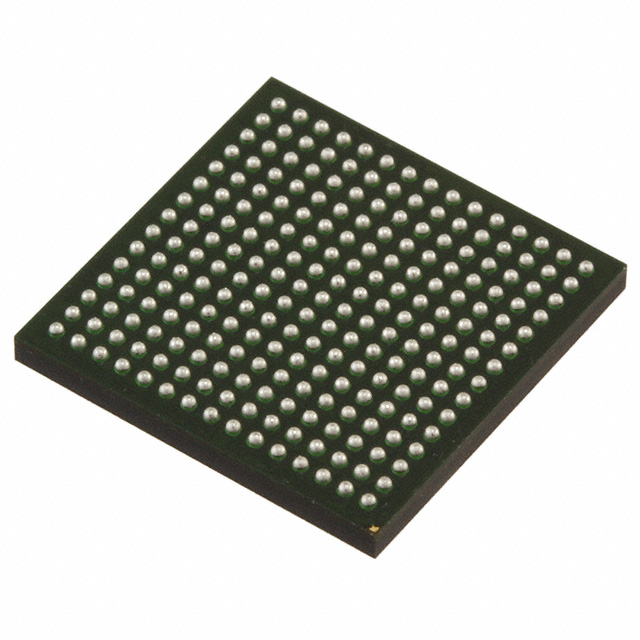
\includegraphics[width=.75\textwidth]{media/CLG225.JPG}
    \caption{CLG255, a 15-by-15 pin BGA package used by the Zynq-7000 series SoC's \cite{clg225}}
    \label{fig:clg255}
\end{figure}

As the pins are hidden when the package is mounted on a PCB, BGA packages are must be soldered by other methods than classical hand-soldering. Reflow soldering is a popular method for soldering BGA's where the entire package and adhering PCB are heated to the point where all the solder melts. This is typically performed in a dedicated reflow soldering oven, but can also be performed using a hot-air gun or similar.


\subsection{CAN-FD}

The different embedded systems on the vehicle communicate with each other using CAN-FD. CAN, or \emph{controller area network} is a network bus developed by Bosch. It has been the de-facto standard communication platform for automotive applications since the mid-1990's. An improved version, CAN-FD (flexible data-rate) was released by Bosh in 2012, it differs from CAN in that the body of each message (called \emph{frames} for CAN) are transmitted at a higher frequency than the header and the allowed frame size increases from 8 to 64 bytes. This is the communication bus currently used at Revolve NTNU.

CAN and CAN-FD is a one-to-many bus system where each frame is given an identifier which determines the priority of the frame. When the bus is free, all connected devices can begin transmitting their frame, but the frame with the highest priority will take precedence on the bus. When a frame is transmitted on the bus, any connected device are able to read it. When the frame has successfully been transmitted the bus is again free and a new transmission can begin.

\subsubsection{CAN-FD bus utilization}

Almost all messages sent over the CAN-FD bus are sent at a regular interval. The size of the different messages are also known, this means that we know how long each message will occupy the bus for. These facts means that the frames on the bus can be modelled in the same way as tasks in a rate-monotonic scheduled system, known from real-time theory. This means the standard formula for utilization can be used when analyzing CAN and CAN-FD buses. The equation for utilization $U$ on a bus is given in equation \ref{eq:utilization}. 

\begin{equation}
    U=\sum_{i=1}^N\frac{C_i}{T_i}
    \label{eq:utilization}
\end{equation}

$C_i$ is the execution time and $T_i$ is the execution period for task $i$. In our case this is translated to the time frame $i$ is active on the bus and the period at which it should be transmitted. 


\subsubsection{Maximum utilization}

We can use the \emph{Utilization-based schedulability test} to determine whether all deadlines are met for a set of tasks. The criteria can be seen in equation \ref{eq:utilization_criteria}. It is important to note that this test is sufficient but not necessary. This means that a passing test guarantees all deadlines are met but a failing test does not guarantee missed  deadlines.

\begin{equation}
    U=\sum_{i=1}^N\frac{C_i}{T_i}\leq N\left(2^\frac{1}{N}-1\right)
    \label{eq:utilization_criteria}
\end{equation}

$N$ denotes the number of different tasks being scheduled. Since the number of different messages on the CAN-FD buses is quite high, we might as well look at what happens to the criteria when $N$ goes towards infinity.

\begin{equation}
    \lim_{N\rightarrow\infty} N\left(2^\frac{1}{N}-1\right)=\ln{2}\approx 0.693
    \label{eq:utilization_criteria_calc}
\end{equation}

From equation \ref{eq:utilization_criteria_calc} we can deem that as long as the bus load on each of the CAN-FD buses are below 69.3\%, no messages are lost. This does of course not mean that the vehicle becomes unusable, figure \ref{fig:canfd_load} shows that the load was above the the limit for both buses, and the vehicle worked fine. The embedded systems are naturally made to be resilient to frame loss.

However, the limit serves as a good target for max bus load, and we will work towards lowering bus load to below this limit.




The high load on the CAN-FD buses poses one of the big challenges with the current system. We want a mathematical model of the load on the CAN-FD buses which can tell us whether messages will be lost or not.

\subsubsection{Rate-Monotonic Scheduling}

As the messages sent over the CAN-FD buses are sent at a somewhat regular interval, the buses can be modeled as a rate-monotonic scheduled (RMS) system. This is a way to model the scheduling of software tasks when the tasks are run at a set interval and with a fixed execution time. We begin by looking at the equation for utilization used with RMS.



Equation \ref{eq:utilization} shows how utilization is calculated for tasks, i.e. how much of the time that a task executes on a single core processor. 

\subsubsection{CAN-FD utilization}

From the RMS utilization equation we know that we need the execution time $C$ and period $T$ for each task. While the period for each CAN-FD message is easy to determine, the execution time takes slighly more effort.From now on we will call the execution time for a message $m$ the \emph{transmission time} and we will denote it $C_m$. For a standard CAN message it would be sufficient to divide the number of bits in the message by the operating frequency of the bus. This is made slightly more difficult as CAN-FD operates on two different frequencies, one for header transmission and one for data transmission. We can split look at the total transmission time as a sum of the transmission time for each of the frequencies , see equation \ref{eq:canfd_cm}.  

\begin{equation}
    C_m=T_s+T_f
    \label{eq:canfd_cm}
\end{equation}

$T_s$, the transmission time for the message header is a constant number of bits, how it is calculated can be seen in equation \ref{eq:canfd_ts}.

\begin{equation}
    \begin{gathered}
        T_s=\frac{(SOF+ID+r1+IDE+EDL+r0+\frac{BRS}{2}+\frac{CRCdel}{2})\cdot1.2}{t_x}\\+\frac{ACK+DEL+EOF+IFS}{t_x}
    \end{gathered}
    \label{eq:canfd_ts}
\end{equation}

The different equations can be seen in equation \ref{eq:canfd_tf}.

\begin{equation}
    T_f=\frac{(D_f+\frac{BRS}{2}+ESI+DLC+\frac{CRCdel}{2})\cdot1.2+CRC+BS}{t_y}
    \label{eq:canfd_tf}
\end{equation}

Because of error detection mechanisms defined in the CAN-FD protocol, the transmission time for payloads larger than 16 bytes is different from payloads smaller than 16 bytes. For payloads smaller than 16 bytes the Cyclic Redundancy Check ($CRC$) is 17 bits and the Bit Stuffing ($BS$) is 5 bits. For payloads larger than 16 bits, $CRC$ rises to 21 bits and $BS$ to 6 bits.


\begin{equation}
    U=\sum_m\frac{C_m}{T_m}
    \label{eq:canfd_busload}
\end{equation}

We will also 

To make reflected decisions about the CAN-FD buses on the vehicle, we need mathematical tools to look at the worst case bus load. Equation \ref{eq:canfd_busload} shows the equation we will use to determine the utilization, or load, $U$ on the CAN-FD bus. $C_m$ is the worst case transmission time (WCTT) for a message $m$ while $T_m$ is the period of message $m$, i.e. how often it is transmitted. It is of course necessary to compute the load from each of the different messages on the bus to be able to calculate the load.



WCTT is pretty straight forward to calculate, but it needs some explanation. What separates CAN-FD from CAN is flexible data-rate (FD). This means that the header or metadata of each frame is transmitted at a lower frequency, just like for CAN, but the payload of the frame is transmitted at a higher frequency, here called $t_y$, while the slower transmission rate is called $t_x$. The total WCTT for a message can be seen as a sum of the worst case time for the header transmission and the higher speed payload transmission, see equation \ref{eq:canfd_cm}.


\subsection{Differential signalling}

When dealing with high-speed, low-power signals in electronic systems, minimizing noise is of the utmost importance. One technique for dealing with this is \emph{differential signalling}. Simply put, it means driving two conductors instead of just one. Single-ended signalling, the conventional method, means that signalling lines are referenced to a common ground. In differential signalling, two lines are used for each signal line. These lines are referenced to each other instead of to a ground shared by all signals. This serves to remove noise that might be present on the ground plane and, when the two conductors are placed close to each other, excellent protection against external interference. When the lines are close to each other, electromagneting fields that normally would introduce noise to the signal will optimally affect both conductors by the same amount, and since we only look at the difference between the two lines, the noise is elegantly subtracted away.

\section{Method}

This section covers the choices made during the design of VCU20. Each subsection takes on a different challenge encountered in the 2019 season.

\subsection{System-on-Module}

The Zynq-7000 platform provided a sufficient platform for running the VCU control loop and the TV algorithm. However, the Zynq-7000 SoC product line are only available in BGA packages. This introduced unwanted complexity to the design, both in term of requirements to the PCB manufacturing, and to the assembly of the PCB, which is a process that normally is performed by team members at the electronic workshop at Revolve NTNU's headquarters. 

In regards to the PCB production process, the BGA package of the SoC adds two kinds of complexity to the design. The first is the need for very tight tolerances. To be able to properly extract all necessary signals from the SoC, a trace width of $0.1\si{\milli\metre}$ is needed. Secondly, a higher number of PCB layers are needed. This is mainly because the SoC requires multiple different supply voltages, $1\si{\volt}$, $1.8\si{\volt}$ and $3.3\si{\volt}$ in the case of Zynq-7010. Both these requirements increase the price of PCB production drastically. Although PCB production houses have increased in number over the last few years, thereby driving the manufacturing cost down, special production techniques like more than 4 layer PCB's and $0.1\si{\milli\metre}$ trace widths still introduces high costs to production runs. A quick comparison on pcbway.com shows that 5 PCBs with 4 layers and a tolerance of $8\textrm{mils}\approx0.20\si{\milli\metre}$ and 4 layers costs 49USD to produce, while the same amount PCBs with tolerances of $4\textrm{mils}\approx0.10\si{\milli\metre}$ and 8 layers costs 388 USD. Additionally, the lead time increases from 4-5 days to 7-8 days. While these numbers might be acceptable for a large production run by a large company, it is most definitely an issue for a voluntary student organization like Revolve NTNU. 

The solution to this issue is to employ as System-on-Module. Instead of mounting the SoC directly on the VCU20 PCB, we can purchase off-the-shelf SoC modules. These modules consists of a small PCB featuring a SoC and some peripherals like external DDR RAM and non-volatile flash memory. The modules interconnects with the VCU PCB by one or more PCB connectors which are easier to route. The downsides to using these modules is mainly the cost. The module utilized for VCU20, Enclustra Mercury ZX5 with Zynq-7015 (figure \ref{fig:zx5}), has a unit price of 318USD. However, as they are modular, they can easily be reused between seasons. Reusing soldered ICs is not common practice at Revolve NTNU, so this should mitigate the high entry cost at least to some extent.

\begin{figure}[H]
    \centering
    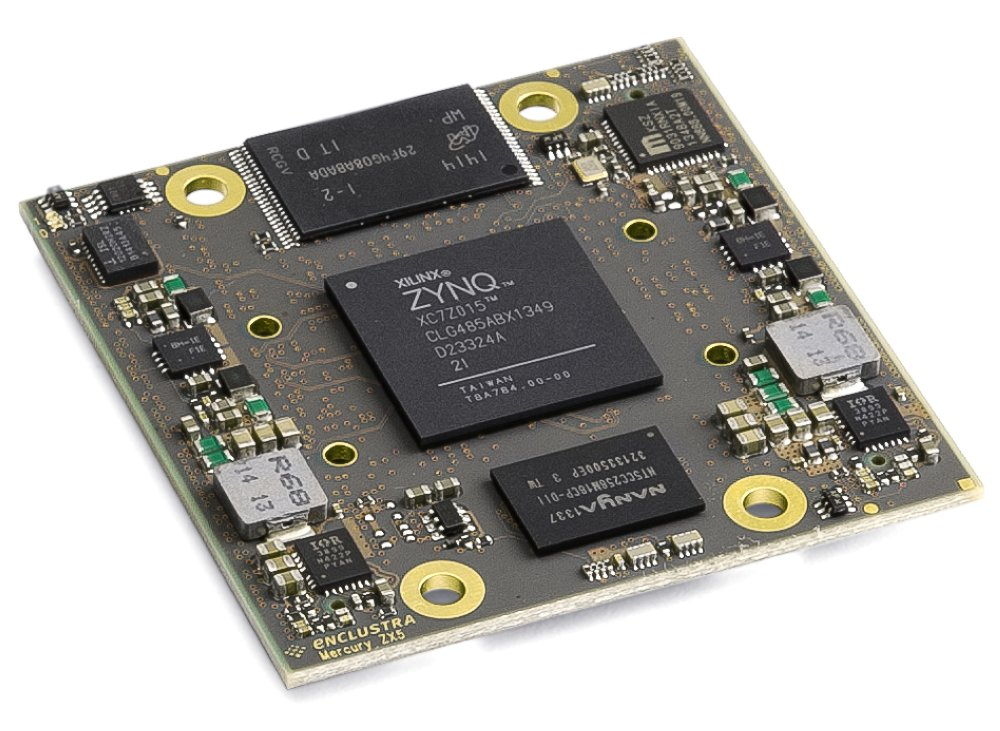
\includegraphics[width=.75\textwidth]{media/zx5.jpg}
    \caption{Enclustra Mercury ZX5 SoM}
    \label{fig:zx5}
\end{figure}

but at the cost of high design complexity. By utilizing a Zynq-7000 based System-on-Module (SoM), we avoid the hard parts of PCB layout, and simply design the VCU as a \emph{breakout board} for the SoM. Using a SoM also gives us access to peripherals that would have been difficult to implement by ourselves, specifically Ethernet, external flash memory and external double data-rate (DDR) memory.

\subsection{Partitioning interfaces}


As the VCU is an integral part of the EV, issues regarding the vehicle are also issues for the VCU. This section is dedicated to some of the issues encountered during last season, which hopefully can be solved by improving the design of the VCU.


In Nova, the main communication channel for the embedded systems were two CAN-FD buses running at a base frequency of 1MHz and an data transfer frequency of 4MHz. A system overview can be seen in figure \ref{fig:vcu19_system}.

\begin{figure}[h!]
    \centering
    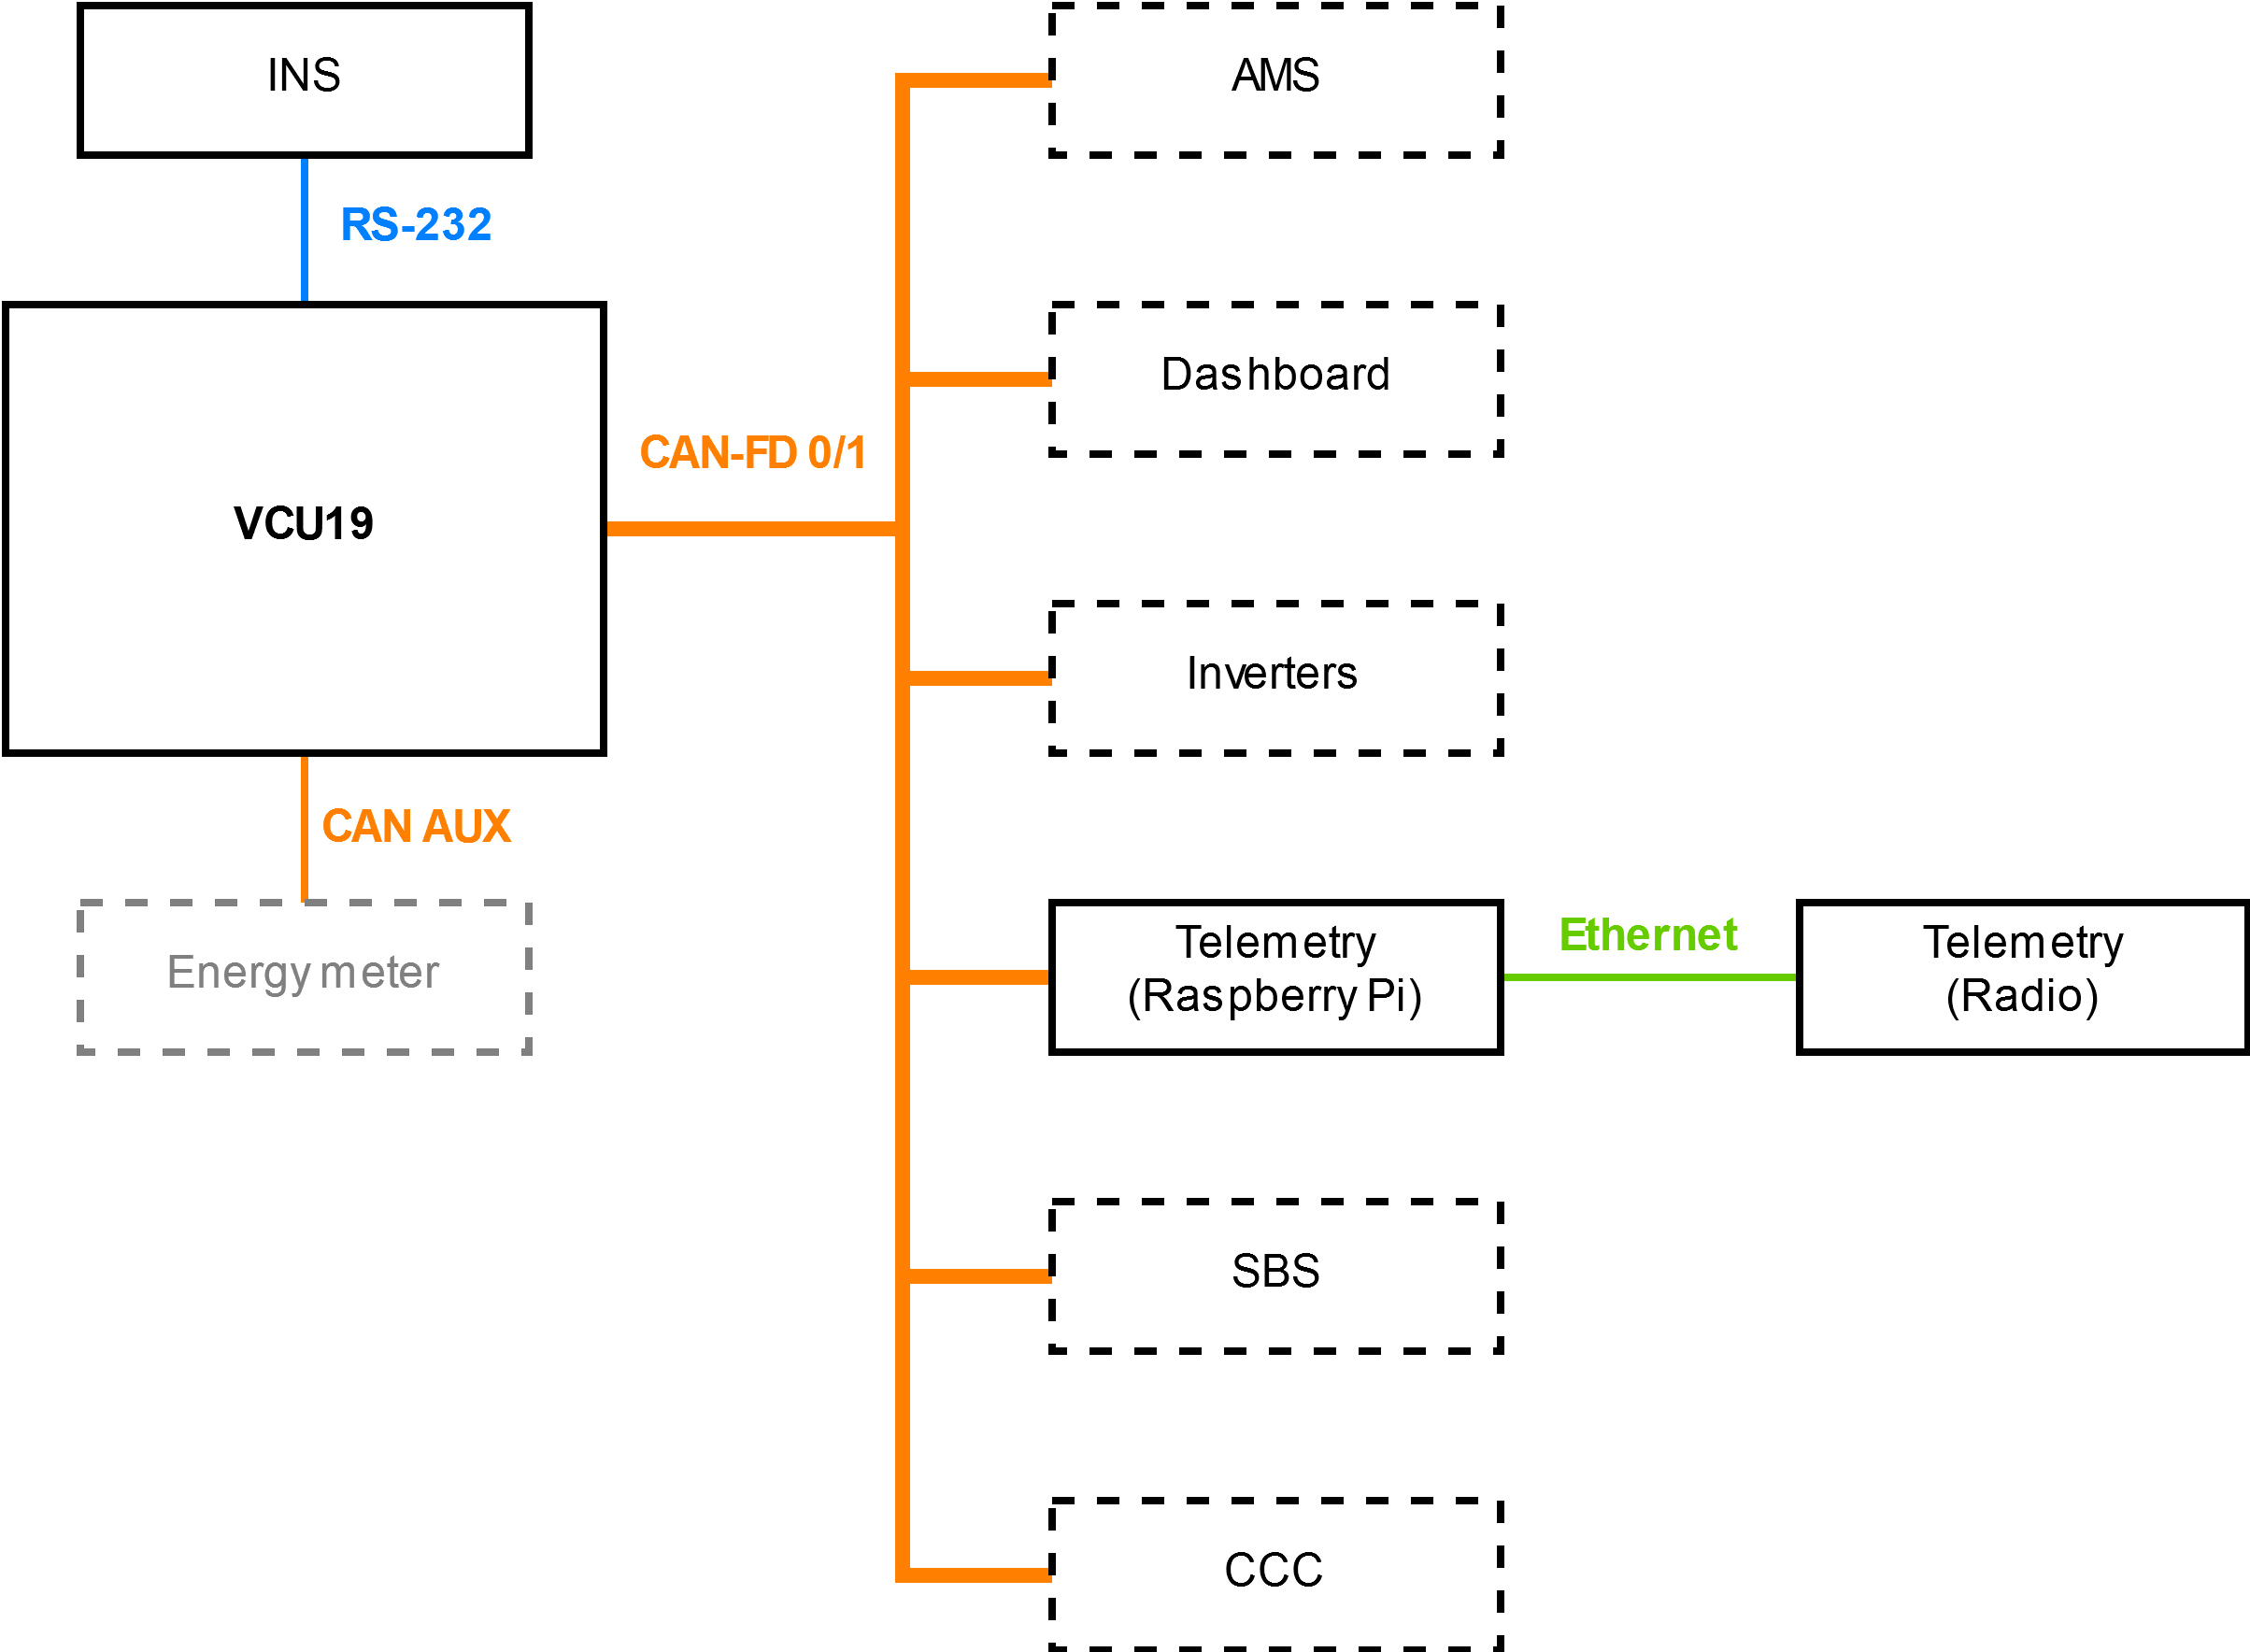
\includegraphics[width=.85\textwidth]{media/vcu19_system.png}
    \caption{VCU19 interface overview. Systems developed by other team members have dotted borders.}
    \label{fig:vcu19_system}
\end{figure}

There are several points where this system can be improved. They will be discussed in detail in the following subsections.


\subsection{Partitioning CAN-FD buses}

A trace of the load on both CAN-FD buses during normal operation can be seen in figure \ref{fig:canfd_load}. Note the increase in load on bus 1 halfway into the trace. This is caused by the car entering "Drive-enable mode" where the VCU starts transmitting set points to the inverters.

\begin{figure}[h!]
    \centering
    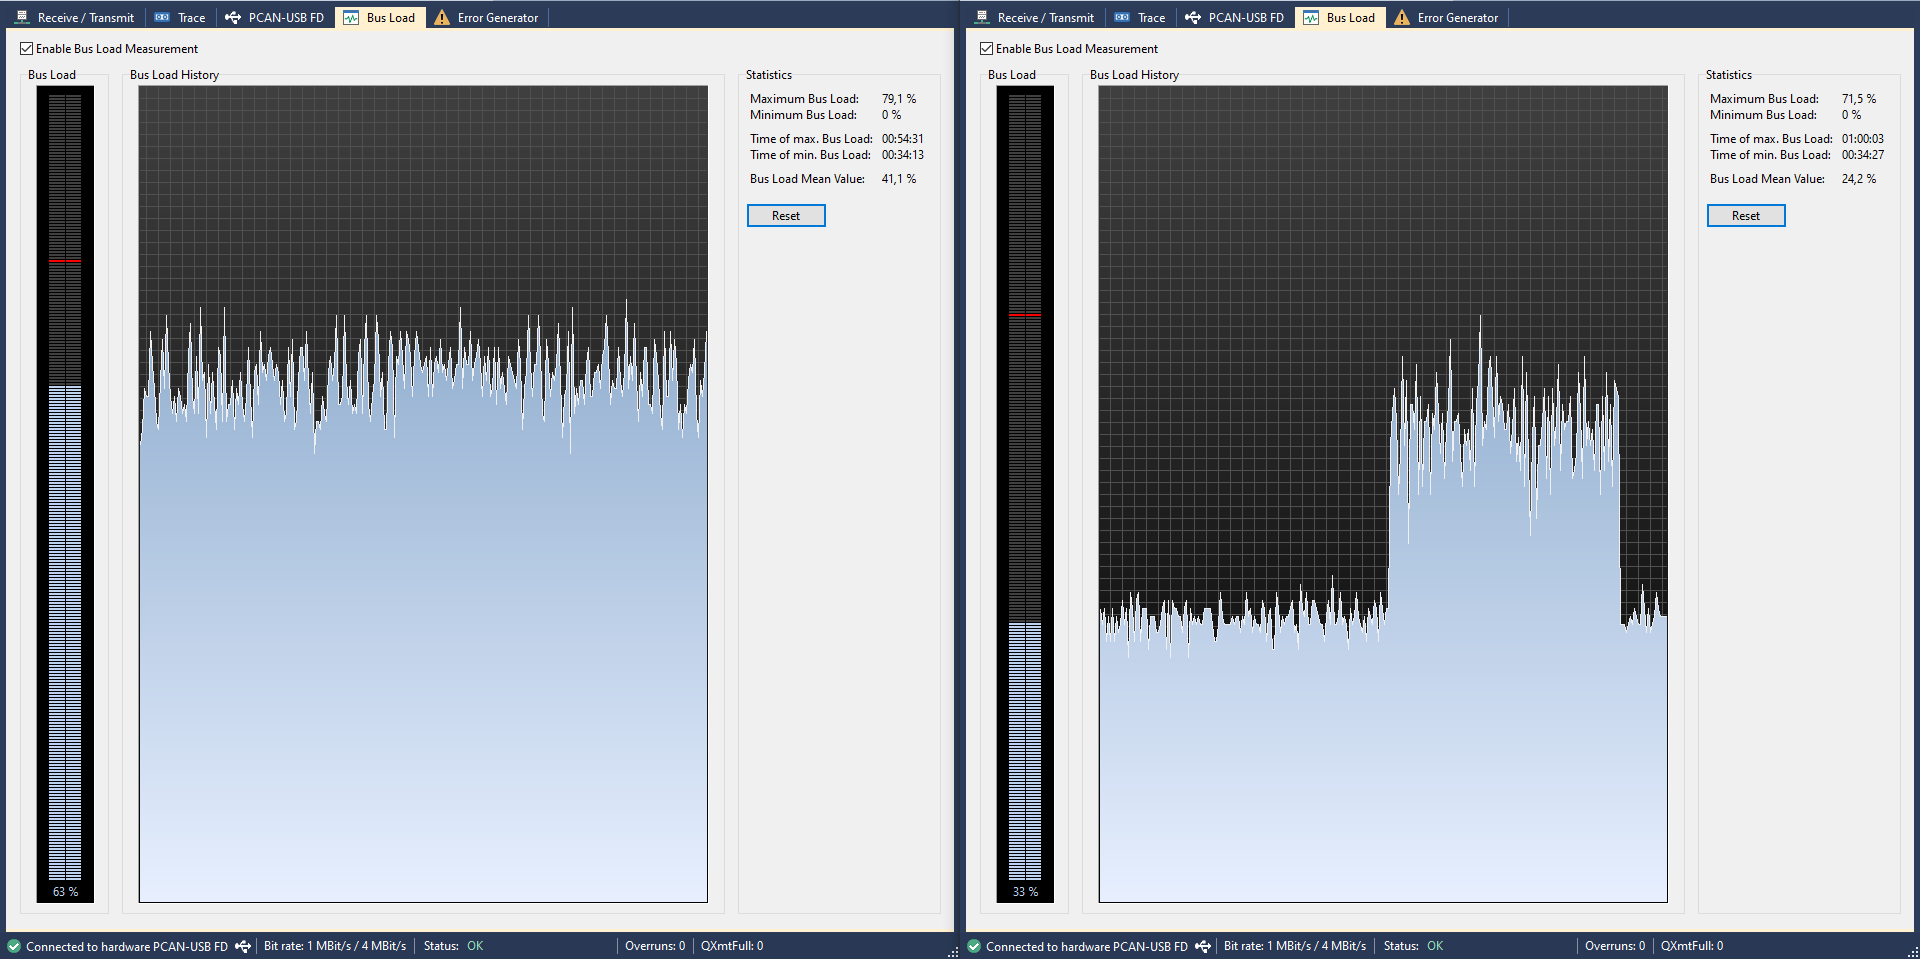
\includegraphics[width=.85\textwidth]{media/canfd-load.png}
    \caption{CAN-FD bus load during typical operation}
    \label{fig:canfd_load}
\end{figure}

From the calculations in section \ref{sec:max_util}, we know that to ensure that no frames are dropped (i.e. all deadlines are met) the bus utilization should be no more than 69\%. For bus 1, this seems to be in order. The trace tells us that the peak utilization is 71.3\%, but this is an outlier and probably not an issue. However, bus 0 seems to have a somewhat high bus load continuously, staying around 70\% load with peaks as high as 79.1\%. This is an area that can be improved.

To start of, we will take a closer look at the frames that are transmitted on each bus. Last season, the team started the process of transitioning from an in-house protocol on top of CAN/CAN-FD (called the Revolve Protocol), to a standardized alternative, UAVCAN. One of the benefits of using UAVCAN is a simplified message definition process. Messages are defined in document schema definition language (DSDL) files and can be converted to C for use in embedded systems and high level data formats like JSON for use in analytics software. As a part of this transition, a simple Python script for calculating the load on each bus based on message size and period was written by Åsmund Eek, a team member from last year that was responsible for the CAN/CAN-FD systems. This code was slightly modified to fit the purposes of this report. 

{\color{red}Calculations on bus load for different systems and different CAN-FD partitioning}

Summing up, a system overview of VCU20 can be seen in figure \ref{fig:vcu20_system}.

\begin{figure}[h!]
    \centering
    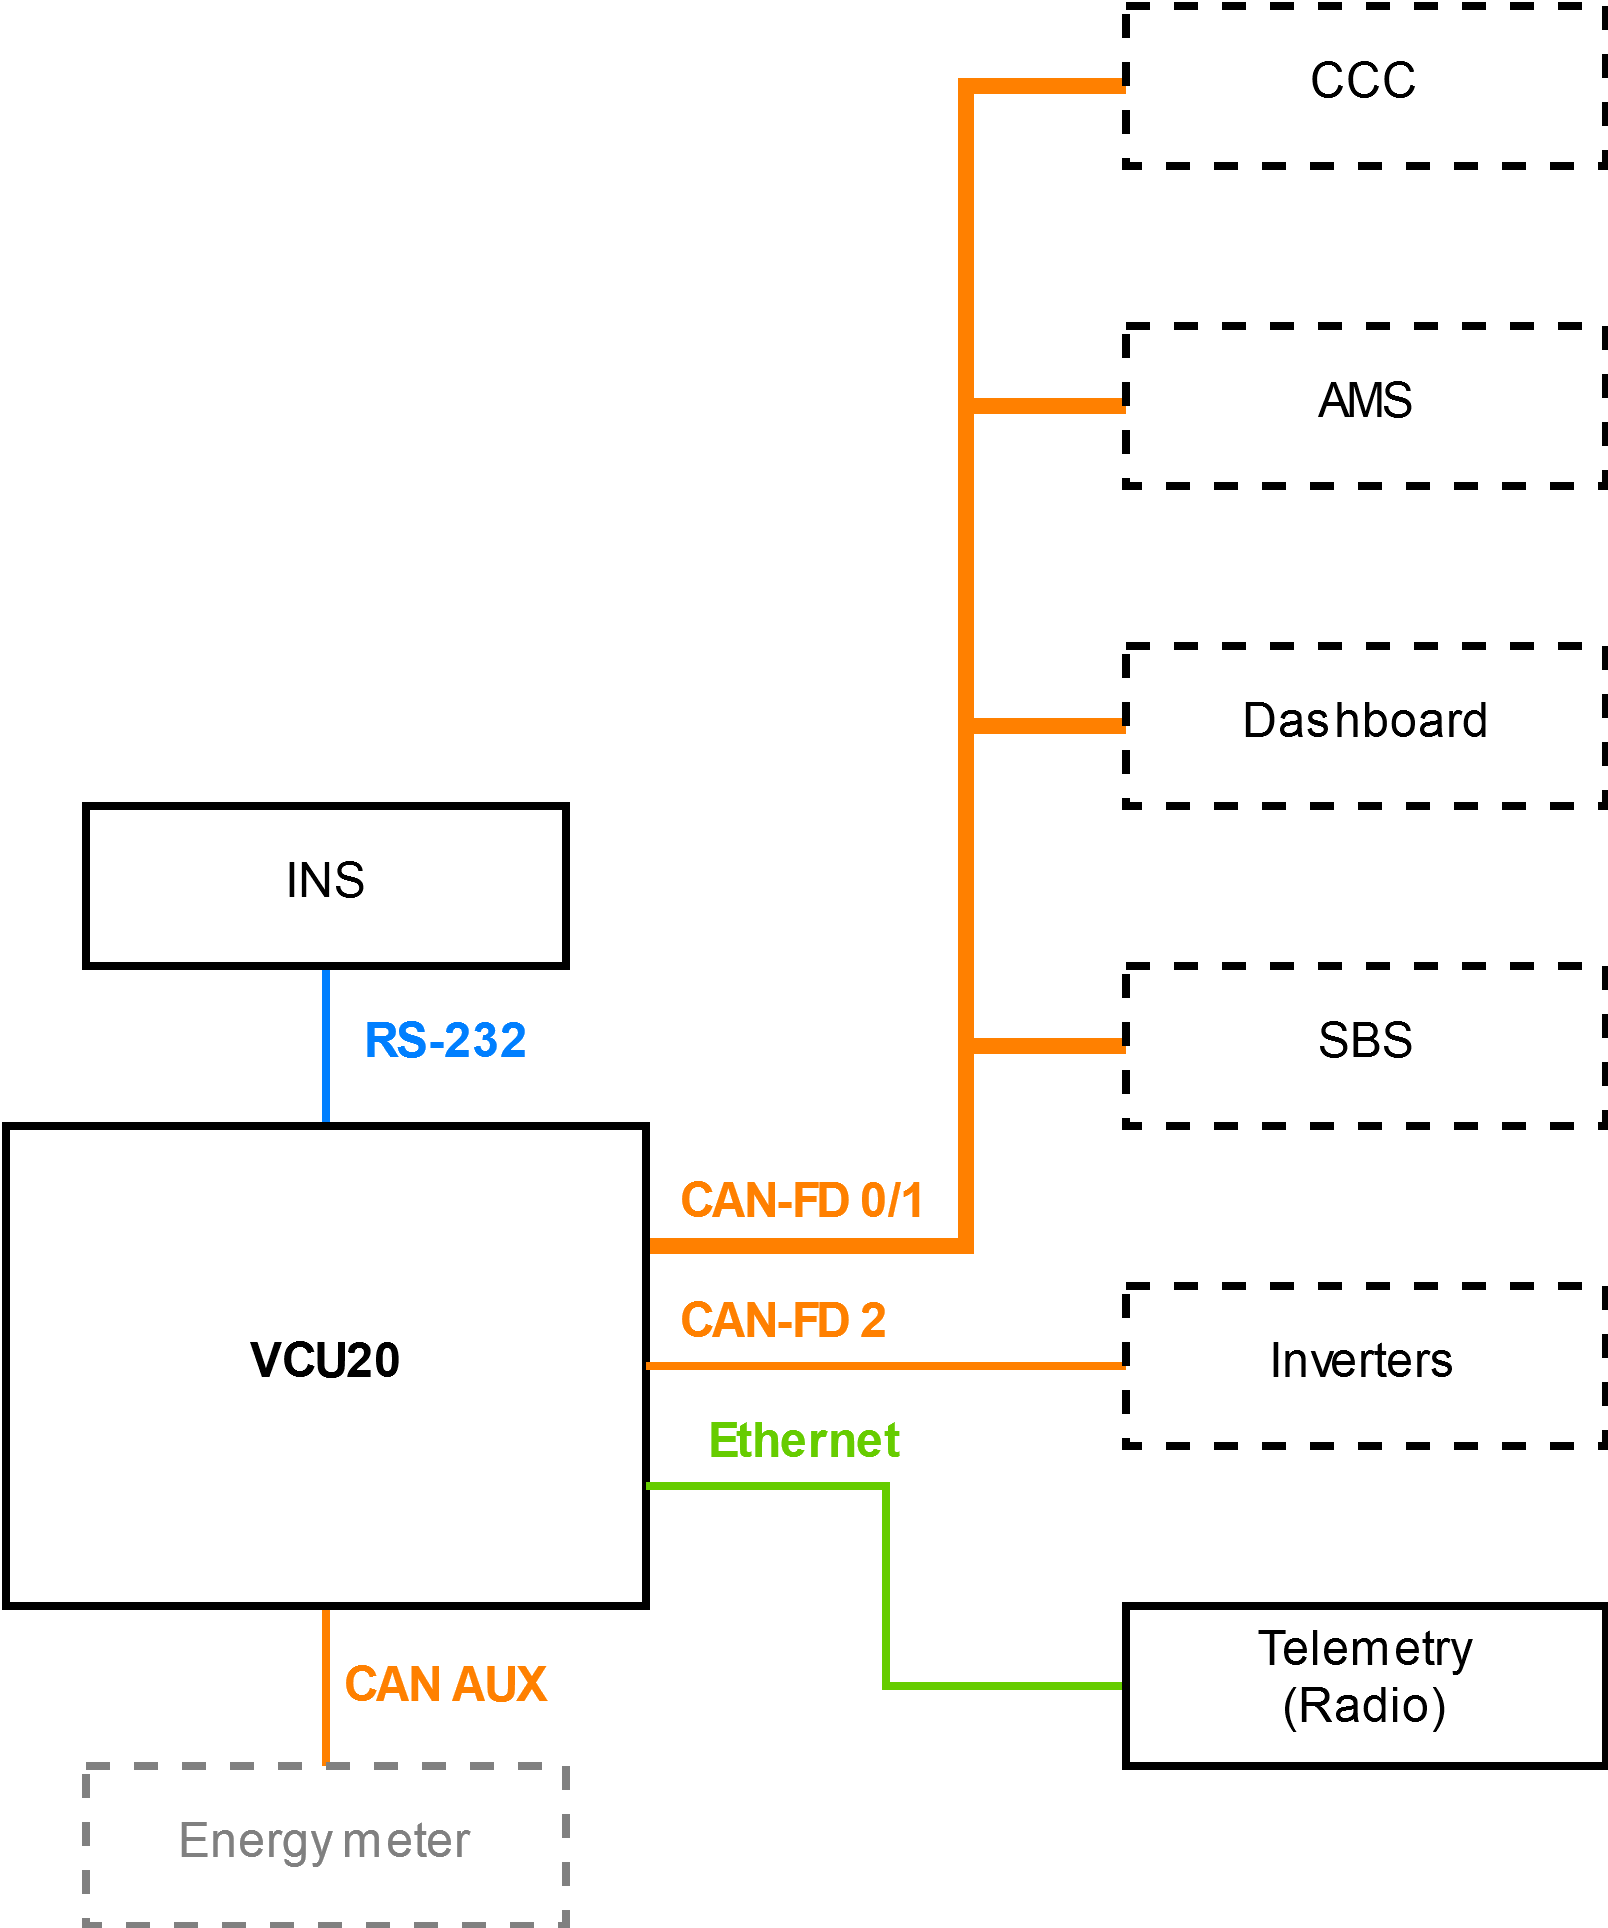
\includegraphics[width=.65\textwidth]{media/vcu20_system.png}
    \caption{VCU20 interface overview}
    \label{fig:vcu20_system}
\end{figure}


%As we want to reduce the load on the CAN-FD buses, we should look closer into ways to partitioning the communication channels in a different way, even add communication channels where that might be applicable. 

%The inverter is heavily dependent on the VCU, but not many other systems. Having a dedicated communication channel between these two systems could potentially reduce the load on the CAN bus by a lot.


%A major issue with the embedded systems on last years EV is the load on the CAN-FD buses. The vehicle is equipped with 2 buses which are shared between all embedded systems on the car. From the bus load analysis in Figure \ref{fig:canfd_load}, it appears that the first bus has a peak of 80\% load, and the second bus peaks at 70\% when under load. The sudden jump in load on the second bus happens when the vehicle enters \emph{drive enable mode}, i.e. when the VCU starts transmitting data to the inverters that drive the motors. This suggests that data going to and from the VCU accounts for much of the total load on the buses. This can be verified by examining the CAN message overview, see figure ... 

%From the aforementioned numbers we can see that much of the data 


\subsection{Ethernet for telemetry}

It is necessary to retrieve data on the vehicle and the different systems on it during races. This is both for later analysis and to indicate to the team if there might be issues with the vehicle before things go wrong. To achieve this, Nova utilized a wireless communication solution from Radionor, the CRE2-144-LW \cite{radionor}. UDP is used to interface with the radio and the physical layer is Ethernet. As no other system on Nova was equipped with Ethernet, the solution was to place a Raspberry Pi 3 B+ in the vehicle, and connect it to the CAN-FD buses with two PCAN-FD USB dongles. The Raspberry Pi would simply gather all available data from the CAN-FD buses and transmit it to the radio over Ethernet. 

As the SoM chosen for VCU20 is equipped with an Ethernet-PHY interface, it is an opportunity to greatly simplify the telemetry system. By connecting the VCU directly to the radio directly using Ethernet, the total weight and complexity of the vehicle can be reduced. The downside to this is that the complexity is moved to the VCU, as it now has to communicate with the radio in addition to everything else. 

It is important that the telemetry system is able to perform at least as well as in Nova. As the previous telemetry system gathered data from both CAN-FD buses and sent the information over Ethernet to the radio, we must consider the bandwidth of both CAN-FD and Ethernet. The buses on Nova ran with a maximum data rate of $4\si{\mega\hertz}$, although it does not use this data rate all the time, we can simplify and say it has a bandwidth of $4\textrm{Mbps}$. This means a total bandwidth of both CAN-FD buses of $8\textrm{Mbps}$. The Raspberry Pi 3 B+ has a maximum Ethernet bandwidth of $300\textrm{Mbps}$ \cite{rpi}. This means the Ethernet interface on VCU20 has to achieve a minimum bandwidth of $8\textrm{Mbps}$. According to the specifications, the Mercury ZX5 module is capable of Gigabit Ethernet ($1 \textrm{Gbps}$) \cite{zx5}. However, the actual speed of the interface is heavily dependent on the quality of the PCB layout. Gigabit Ethernet consists of four differential pairs, each of which should be matched in length to each other and within the pair to achieve maximum bandwidth.


% Looking at the messages which are being transmitted be the telemetry system, it is evident that much of the data originates from the VCU. However, most of this data does not need to be read by any other embedded system on the vehicle. A great improvement from last seasons design would therefore be to add an Ethernet interface to the VCU. This should reduce the load on the bus by a lot.



\section{Results}

\subsection{CAN-FD bus partitioning}

{\color{red} Calculations on bus load for 2 and 3 buses}

\subsection{CAN-FD interface performance}

{\color{red} Benchmark of CAN-FD speed, make sure it performs as well as necessary (from calculations)}

\subsection{Ethernet speed}

{\color{red} Benchmark Ethernet interface bandwidth. Calculations showing wether it is able to transmit all data from CAN-FD buses over telemetry}


\section{Discussion}

\subsection{PCB design}

The use of hierarchical design made the \acrshort{pcb} design process relatively simply. Layout of the Ethernet interface required use of differential signalling, this is the most complex piece of hardware design in this project. Because of tools made specifically for this kind of work in the \acrshort{pcb} layout software, this process is made easier even for inexperienced hardware designers.  

\subsection{PCB production}

It is worth noting that the prototype production run of \acrshort{vcu20}, a sponsor of Revolve NTNU covered all costs of \acrshort{pcb} production. This renders the argument of reducing cost by employing a \acrshort{som} somewhat moot. However, this has not been the case for previous teams, and it is far from certain that it will continue like this in the future.

\subsection{PCB assembly}

Soldering the finished \acrshort{pcb} was done solely by hand without any major problems. The connectors used for the ZX5 module has a \emph{pitch} (distance between the individual pins) of $0.5\si{\milli\metre}$, which is hard to solder by eye. A microscope was used for this part of the soldering, and since Revolve NTNU owns several microscopes this is not regarded as a large issue.   

\subsection{PCB testing}

When soldering was finished, \acrshort{vcu20} underwent a series of tests to ensure correct design and assembly. This is a necessary part of any engineering design process and it was able to uncover one rather large mistake in the design of \acrshort{vcu20} which rendered the \acrfull{jtag} interface necessary for flashing firmware onto the \acrshort{som}, unuseable. Luckily, it was possible to correct this error by unsoldering a buffer intended to protect the programming interface from noise when inside the \acrshort{ev} and soldering jumper wires to the pads.



\printbibliography

\newpage
\section*{Appendix}

\subsection*{Layout}

\subsection*{Schematics}

\subsection*{CAN-FD calculations}

{\color{red} Also including source code}

\subsection*{Benchmarks}


% Note: jeg må bruke flere ord
% Være litt mer utfyllende

% Benchmark noe som er lett å benchmarke
% Husk å være litt kritisk til modulen

% Tidsplan er smart

\end{document}